\chapter{Literature Study}
\label{chp:litreview}


\begin{figure}[htb!]
    \centering
    \input contents/chapt2/figs/literature_taxonomy_sections.tex
    \caption[A taxonomy of the autonomous racing literature with sections]{A taxonomy of the autonomous racing literature. The blue leaf nodes reference the section relevant to their description.}
    \label{fig:my_neuron}
\end{figure}

\section{Classic Pipeline}
\label{sec:classic}

\subsection{Trajectory planning}
\label{sec:trajectory_planning}

\begin{figure}[h]
    \centering
    \includegraphics{contents/chapt2/figs/classic_pipeline_planning.png}
    \caption{The classic autonomous driving pipeline with the trajectory planning modules relevant to this section colored in blue.}
    \label{fig:trajectory_planning}
\end{figure}

Global trajectory planning
geometric
\cite{Braghin2008} - shortest path vs minimum curvature

optimisation
\cite{Herrmann2019} - energy management
\cite{Herrmann2020} - optimization includes power usage of battery

genetic algorithms
\cite{Cardamone2010}
\cite{Vesel}

Local trajectory planning
\cite{Liniger2015a} - viability kernel for safe set of states
\cite{keefer2022} 
\cite{Wang2021}
\cite{Jeon2013} - a* shortest path search

\subsection{Control}
\label{sec:control}

\begin{figure}[h]
    \centering
    \includegraphics{contents/chapt2/figs/classic_pipeline_control.png}
    \caption{The classic autonomous driving pipeline with the control modules relevant to this section colored in blue.}
    \label{fig:control}
\end{figure}

classic control

geometric control
latitude control
\cite{Coulter_1992} pure pursuit
\cite{Hoffmann2007} Stanley control

gg diagram
\cite{talvala2011} stabilise with lyapunov, use gg diagram

latitude and longitude control
\cite{Kritayakirana2010} gg diagram control


model predictive controllers

\cite{Pup2020} - characterising uncertainty in vehicle models from linearisation
\cite{Beal2013} - vehicle stabilisation at limits of handling
\cite{Liniger2019} - viability kernel to limit search space
\cite{Williams2016} - model predictive path integral control  
\cite{Hewing2018} - control cars under model inaccuracy with learning non-linear mpc

learning based control
\cite{Ji2018}
\cite{Brunner2018a}

\subsection{Full driving stacks}
\label{sec:full_driving_stacks}

\begin{figure}[h]
    \centering
    \includegraphics{contents/chapt2/figs/classic_pipeline_full_stack.png}
    \caption{The classic autonomous driving pipeline.}
    \label{fig:full_stack}
\end{figure}

\cite{Valls2018}
\cite{sherif2020}
\cite{Wischnewski2019} - kinematic state estimation
\cite{Vazquez2020} - in global planning
\cite{alvarez2022}

\section{End-to-end pipeline}
\label{sec:end_to_end}

The limitations of classical methods has led to research in learning-based systems that improve the vehicle dynamics model or action policy with real-world data and allow more complex cost formulations and non-linear dynamics \cite{Fuchs2021}.
Many learning approaches use an end-to-end pipeline, illustrated in Figure \ref{fig:end_to_end}, whereby a single neural network predicts control outputs from sensor data.
The neural networks used in end-to-end approaches are typically trained using imitation or reinforcement learning paradigms \cite{Betz2021}. We present a summary of research efforts into both approaches.

\begin{figure}[h]
    \centering
    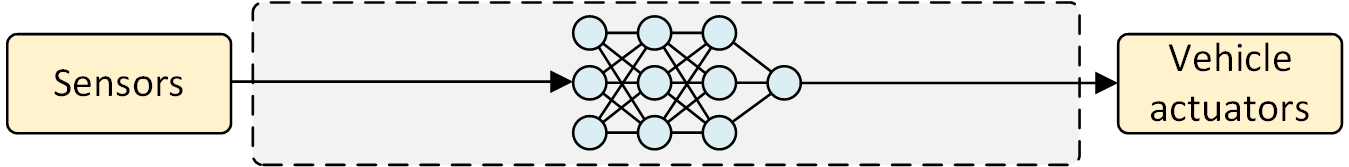
\includegraphics{contents/chapt2/figs/end_to_end_pipeline.png}
    \caption{The end-to-end autonomous driving pipeline.}
    \label{fig:end_to_end}
\end{figure}

\subsection{Imitation learning}
\label{sec:imitation_learning}

Imitation learning techniques train a neural network to mimic an expert such as a human or optimisation method.
The process is analogous to supervised learning, where labelled data is used to train an algorithm to predict outcomes on new data.
In the context of autonomous racing, the labelled training data is produced by allowing an optimisation method or human to interact with the vehicle.
This produces a set of control commands which act as the labels for the inputs to the neural network.
Supervised learning is then used to train an algorithm to predict control commands for new data \cite{Osa_2018}.

Imitation learning is the preferred method of training a neural network if it is feasible for an expert to demonstrate optimal behaviour but difficult to define a reward manually.
For instance, in some circumstances where vehicle manoeuvres are complex, correct driving behaviour may be more easily specified by a human demonstrator than manually designing a reward signal.
Furthermore, the expert limits the need for exploration, as required by reinforcement learning \cite{Osa_2018}.

A major benefit of imitation learning with neural networks is the cost of online computation: neural networks are far less computationally expensive to run than optimisation methods. This is demonstrated by Tatulea-Codrean et al. \cite{Tatulea-Codrean2020}, who train a neural network to mimic the policy of a non-linear MPC (NMPC). The NMPC is too computationally expensive for real-time control of the vehicle. 
However, the neural network computes the control command in a much faster time, enabling the deployment of the vehicle.

Imitation learning in conjunction with neural networks also have the benefit of being flexible towards their inputs. Whereas optimisation methods have strict requirements for the input as frequent state and boundary condition updates, imitation learning enables a neural network to learn from high dimensional inputs such as images from a video feed. This is accomplished by Mahmoud et al. \cite{Mahmoud2020} and Pan et al. \cite{Pan2017a}. 
Pan et al. \cite{Pan2017a} showcase the usefulness of this property by using imitation learning to relax hardware requirements and reduce the cost of the vehicle sensor suit. 
Their neural network is trained to mimic an MPC on a vehicle with two sensor suits: an IMU and GPS unit worth 6000\$, and 500\$ camera.
While the MPC requires the 6000\$ IMU and GPS, the neural network is trained to execute the same policy on the 500\$ camera.

The flexibility of neural networks towards their inputs is related to another useful property: robustness to sensor noise and failure. 
This property is showcased well by Lee et al. \cite{Lee2019}, who use imitation learning to create an ensemble of bayesian neural networks (BNN) on different sensor inputs to create a redundant control policy. 
The algorithm is robust to sensor noise and even multiple sensor failures, which was not possible using more traditional optimisation methods.

From these examples we see that imitation learning learning with neural networks is a powerful tool.
However, Wadekar et al. \cite{Wadekar2021} highlight some weaknesses of the imitation learning technique.
The neural network policy will not match the expert policy exactly. 
Since policy affects the distribution of states that the vehicle encounters, the vehicle may encounter a scenario for which no expert training data was generated during training, in which case it is likely to take an incorrect action \cite{Osa_2018}.
Furthermore, Wadekar et al. \cite{Wadekar2021} describe that the data collected by the expert must be curated so that the agent does not learn any undesirable behaviour.
Perhaps the most undesirable characteristic of imitation learning is that it requires expert training data.
This makes it unsuitable for scenarios where expert training data is not available, as in cases where optimisation methods fail \cite{Fuchs2021a}.



\cite{Wadekar2021} 
A shortcoming of IL The data used to train the neural network must be curated by an expert so that undesirable behaviour is not learned.
This is a labor intensive process, as every date instance must be inspected.
Wadekar et al. \cite{Wadekar2021} train a neural network to predict control actions for a simulated car from game images.

to create a driving algorithm that is robust to sensor noise and even failure.

\cite{Lee2019} physical vehicle
Lee et al. \cite{Lee2019} use am ensemble of bayesian neural networks (BNN) to create a driving algorithm that is robust to sensor noise and even failure.
Lee et al. \cite{Lee2019} train multiple BNNs on different sensor inputs to create a redendant control policy.

This is particularly useful when the neural network has access to lower cost sensors, allowing the optimisation method policy to be executed on a cheaper sensor suit \cite{Pan2017}. 
Neural networks trained with imitation learning have also shown greater robustness to sensor failure and faster online execution time \cite{Wadekar2021} than expert optimisation methods \cite{Lee2019}. 
However, imitation learning is not a suitable method for training a neural network policy in scenarios where expert training data is not available, as in cases where optimisation methods fail \cite{Fuchs2021a}.

learned neural networks are trained to mimic an expert such as a human or
optimisation method.

Simulation
\cite{Tatulea-Codrean2020} NMPC for control to imitation learning
Neural networks execute faster than non-linear MPC (NMPC) methods
NMPC methods are too computationally demanding for the on-board hardware found on most small racecars.
The results generated by the NMPC are used as a training data set for a neural network.
The neural network achieves performance competitive with the NMPC. 

\cite{Wadekar2021} 
A shortcoming of IL The data used to train the neural network must be curated by an expert so that undesirable behaviour is not learned.
This is a labor intensive process, as every date instance must be inspected.
Wadekar et al. \cite{Wadekar2021} train a neural network to predict control actions for a simulated car from game images.

\cite{Mahmoud2020} - 
Another benefit of neural networks is flexibility towards changes in sensor input.
This is shown by Mahmoud et al. \cite{Mahmoud2020}, who trained a neural network with a set of scaled down input images.
This was to show that the neural network's response rate increased when using the smaller images.

\cite{Lee2019} physical vehicle
Lee et al. \cite{Lee2019} use am ensemble of bayesian neural networks (BNN) to create a driving algorithm that is robust to sensor noise and even failure.
Lee et al. \cite{Lee2019} train multiple BNNs on different sensor inputs to create a redendant control policy.


Physical
\cite{Pan2017a} - does not require state estimation or online optimisation for planning
The flexibility of neural networks is further demonstrated by Lee et al. \cite{Pan2017a}
who train a imitation learning algorithm on a vehicle with two sensor suites.
One sensor suit is an IMU and GPS unit worth 6000\$, the other is a camera worth less than 500\$.
An MPC uses the IMU and GPS to compute a policy. 
However, the neural network learns a to imitate the MPC using video footage from the camera.
Neural networks can learn from high dimensional data sets such as images.
this is useful, as cameras are widely available and generally cheaper than sensor suits required by classical methods.


\subsection{Reinforcement learning}
\label{sec:reinforcement_learning}

Reinforcement learning approaches may be categorized according to whether they use a model to plan or simply learn from past experience
two rl paradigms

Model based learning
simulation
\cite{Schwarting2021} - Deep Latent Competition: Learning to Race Using Visual Control Policies in Latent Space
Racing is challenging when multiple vehicles compete in the same environment
this requires fast processing of observations and seasoning about opponents behaviour
multi-agent settings, behavioral and environmental features may be too complex to be captured by MPC or purely game-theoretic approaches that assume perfect knowledge of the state and the system dynamics.
Deep Latent Competition learns a world model for imagining competitive behavior in latent-space

Highlights a major advantage of using reinforcement learning: complex cost formulations and the ability to make a decision while
partial observability of other agents
Algorithm is deployed in openAI gym racecar environment
learns on a birds-eye view of the track 

most variations of MPC rely on tools from constrained optimization, which means that convexification (such as with quadratic approx- imation) of the cost function and first or second order approximations of the dynamics are required.
A more flexible MPC method is model predictive path
integral (MPPI) control, a sampling-based algorithm which can optimize for general cost criteria, convex or not. However, in prior work, MPPI could only be applied to systems with control affine dynamics.

physical deployment
\cite{brunnbauer}
We demonstrate the effectiveness of advanced model- based deep RL compared to model-free agents in the real-world application of autonomous racing.
Brunnbauer deploy the model-based Dreamer reinforcement learning algorithm by Hafner et al. \cite{Hafner2019a} on a physical F1tenth vehicle.
Learns an observation model, dreamer learns a policy purely on imagined sequences without interaction with the environment, resulting in safe and data-efficient learning
Outperforms model-free approaches by travelling further

\cite{Williams2017}
Relaxes the assumption that MPPI can only be applied to systems with linear dynamics.
Derive an update law to MPPI that is applicable to stochastic systems
by combining  model predictive control with model-based reinforcent learning.
This enables a purely data-driven approach to model learning in MPPI framework.
Vechile dynamics model is learned with MPPI 
Test controller  on a physical vehicle on a gravel track.
Vehicle performs well and is capable of performing aggressive driving manoeuvres on a gravel track. 

Model free 
Simulation 

Perot et al. \cite{Perot2017} and Jaritz et al. \cite{Jaritz2018} present pixel to control algorithms for racing in the video game World Rally Cross 6.
Both approaches utilise a convolutional neural network (CNN) with long short-term memeory (LSTM). Jaritz et al. \cite{Jaritz2018} state that a score given at the end of the race is too sparse for the agent to learn effectively, introducing a continuous reward schema involving a reward proportional to the vehicle's velocity, and a penalty proportional to the cross track and heading error (the distance between the vehicle and closest centerline point, and the difference between the vehicles heading and the heading of that same point).
Both approaches show that pixel to control is both extremely inefficient and unsafe; Both Jaritzet al. \cite{Jaritz2018} and Perot et al. \cite{Perot2017} train their agent for 80 million steps.
crashes per kilometer


State of the art
\cite{Fuchs2021}
Fuchs et al. \cite{Fuchs2021} presents a soft actor-critic (SAC) agent that achieves lap times on par with competitive e-sports drivers in the racing game Gran Turismo Sport.
Key to their approach is careful selection of hand-crafted input features that include: 1) the vehicles velocity $\pmb{v}_t \in \mathbb{R}^3$, 2) acceleration $\pmb{\dot{v}}_t \in \mathbb{R}^3$, 3) distance measurements of $M$ rangefinders $\pmb{d}_t \in \mathbb{R}^M$, 4) the previous steering command $\delta_{t-1}$, 5) a binary flag indicating wall contact, and 6) $N$ sampled curvature measurements of the track centerline $\pmb{c}_t \in \mathbb{R}^N$.

Also introduce a continuous progress term into the reward signal, whilst penalising the agent for making contact with the track boundary

\begin{equation}
    r_t = r_{t}^{\text{progress}} - 
    \begin{cases}
    c_w \| \pmb{v}_t \| & \text{if in contact with wall} \\
    0 & \text{otherwise.}
    \end{cases}
\end{equation}

Although their implementation remains in simulation, Fuchs et al. \cite{Fuchs2021} do measure the effect of vehicle model inaccuracies by changing the parameters of the vehicle model between training and testing. They find that increased tire friction causes the agent to steer more aggressively leading to brief contact with the inside wall. A decrease in tire friction causes the agent to take corners slightly wide resulting in contact with the outside.
They also measure the effect of delays to the agents inference, finding that delays of greater than 100ms leads to track boundary contact. 
From Fuchs et al. \cite{Fuchs2021} it is not clear what degree of model inaccuracy results in collisions.

Remonda et al. \cite{Remonda2021} perform a similar study as Fuchs et al. \cite{Fuchs2021}, training an agent with similar hand-crafted features and reward signal to race alone in The Open Racing Car Simulator (TORCS). They report that their agent learns similar behaviour policies as professional racing drivers.

\cite{Song2021}
Song et al. \cite{Song2021} extends the work from Fuchs et al. \cite{Fuchs2021} to a multi-agent setting, training an agent to overtake other vehicles.
key to their success is the use of curriculum learning, whereby the agent is trained to solve increasingly difficult tasks by adding components to both the environment and reward signal. 
The agent is trained to race on its own before another vehicle is added to the simulation, and the reward signal is modified to encourage the agent to make progress relative to the other vehicle.
Showcase the strength of reinforcement learning: While optimisation algorithms rely on the convexification of cost functions, reinforcement learning agents can learn to solve difficult tasks from complex cost functions.

We move away from now games and discuss approaches that more directly address the sim2real gap.
\cite{Niu2020} - curriculum learning + safety controller
Niu et al. \cite{Niu2020} propose a model-based safety controller that acts as a safeguard mechanism, preventing the agent from selecting unsafe actions.
They foresee that the safety module's reliance on an accurate vehicle model is an issue. 
As such, a neural network is used to learn a vehicle model online that eventually replaces the assumed vehicle model.
The safety controller allows the policy to converge faster and more robustly.



Physical deployment + sim2real gap

\cite{hsu2022}
Hsu et al. \cite{hsu2022} identify control smoothness as an issue with the deployment of reinforcement learning onto physical vehicle vehicles. 
Sudden control actions will induce excessive mechanical wear and cause the vehicle to exhibit dangerous behaviour.
They apply Conditioning for Action Policy Smoothness (CAPS) to smooth the control action of the vehicle.
Although Hsu et al. \cite{hsu2022} do not directly address model inaccuracies, their policy smoothing approach produces a conservative policy which is expected to increase performance and safety in settings where the model in inaccurate.


\cite{Chisari2021}
Chisari et al. \cite{Chisari2021} deployed a soft actor-critic model-free reinforcement learning algorithm onto a physical vehicle.
They make the agent policy robust to real-world transfer training in simulation with a slightly randomised vehicle model.
This results in an over-conservative policy.
The agent policy is then refined after the physical vehicle is deployed.
This allows the reinforcement learning algorithms to achieve lap times similar to an MPC controller, while reducing track boundary collisions by half.

\cite{Ivanov2020}
Ivanov et al. \cite{Ivanov2020} take a similar approach to Chisari et al. \cite{Chisari2021} by training an agent with model randomisation, but are not able to achieve robustness to the sim2real transfer.


\section{Partial end-to-end pipeline}
\label{sec:partial_end_to_end}

\begin{figure}[h]
    \centering
    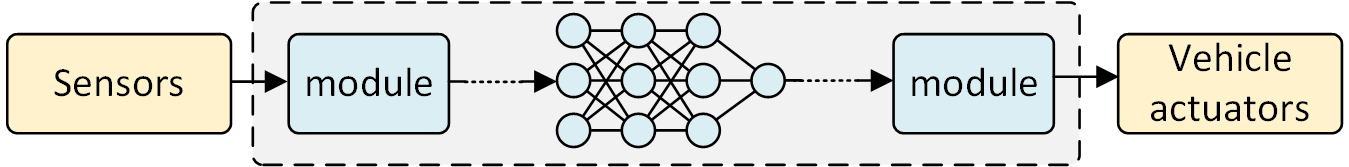
\includegraphics{contents/chapt2/figs/partial_end_to_end_pipeline.png}
    \caption{The partial end-to-end autonomous driving pipeline.}
    \label{fig:partial_end_to_end}
\end{figure}

Reinforcement learning
\cite{Evans2021b} - learning local planning
\cite{Capo2020} - short term trajectory planning using rl
\cite{Ghignone2022} - rl for following trajectory. Outperforms mpc

Imitation learning
\cite{Weiss2020a} - local planning
\cite{Weiss2020}

\begin{landscape}
    \newcolumntype{a}{>{\hsize=1\hsize \centering\arraybackslash}X}
\newcolumntype{d}{>{\hsize=.5\hsize \centering\arraybackslash}X}
\newcolumntype{e}{>{\hsize=2\hsize \centering\arraybackslash}X}


\begin{table}[h]
\centering
\begin{tabularx}{21cm}{|a|d|d|d|d|e|}
    
    \hline
    \small \textbf{Name} & \small \textbf{Model-based} & \small \textbf{Multi-agent} & \small \textbf{Input} & \small \textbf{Physical vehicle} & \small \textbf{sim2real approach} \\
    \hline
    \small Schwarting et al. \cite{Schwarting2021} & \checkmark & \checkmark & \small game image & & - \\
    \hline
    \small Brunnbauer et al. \cite{brunnbauer2021} & \checkmark & & \small features & \checkmark & - \\
    \hline
    \small Perot et al. \cite{Perot2017} & & & \small game image & & - \\
    \hline
    \small Jaritz et al.  \cite{Jaritz2018} & & & \small game image & & - \\
    \hline 
    \small Fuchs et al. \cite{Fuchs2021} & & & \small features & & \small Test effects of model inaccuracy in simulation \\
    \hline
    \small Remonda et al. \cite{Remonda2021} & & & \small features & \checkmark & - \\
    \hline 
    \small Song et al. \cite{Song2021} & & \checkmark & \small features & & - \\
    \hline
    \small Niu et al. \cite{Niu2020} & & & \small features & & \small Safety module based on learned vehicle model prevents agent from selecting unsafe actions. \\
    \hline
    \small Chisari et al. \cite{Chisari2021} & & & \small features & \checkmark & \small Parameter randomisation while training, policy refinement after deployment \\
    \hline
    \small Ivanov et al. \cite{Ivanov2020} & & & \small features & \checkmark & \small Parameter randomisation while training \\
    \hline
    \small Hsu et al. \cite{hsu2022} & & & \small image & \checkmark & \small Control action smoothing \\
    \hline

\end{tabularx}
\caption[A summary of end-to-end reinforcement learning approaches for autonomous racing]{A summary of end-to-end reinforcement learning approaches for autonomous racing.}
\label{table:autonomous_racing_rl_summary}
\end{table} 

    \footnote{The absence of a tick in the model-based, multi-agent , and physical vehicle columns indicate that the approach was model-free, single-agent and simulation only, respectively. \label{footnote_1}}
\end{landscape}